\subsection{Pengujian Komponen \textit{Predictor}}

Pada bagian ini akan dijelaskan tentang tujuan, skenario, hasil, dan analisis dari pengujian komponen \textbf{\textit{Predictor}}.

\subsubsection{Tujuan Pengujian}

Tujuan pengujian ini memastikan komponen \textbf{\textit{Predictor}} memakai model yang menghasilkan data prediksi yang baik dan dapat digunakan.

\subsubsection{Skenario Pengujian}

Pengujian terhadap model prediksi dilakukan dengan \textit{dataset web server logs} NASA selama dua bulan. Data ini dikumpulkan oleh NASA Kennedy Space Center WWW server di Florida selama dua bulan dan bisa diklasifikasikan menjadi dua buah bagian. Bagian pertama dimulai dari 00:00:00 1 Juli 1995 sampai 23:59:59 31 July 1995 dengan total 31 hari. Bagian kedua dimulai dari 00:00:00 1 August 1995 sampai 23:59:59 31 August 1995. Kedua bagian ini mengandung $3.461.612$ permintaan secara total. Karena adanya badai Erin, server ditutup, sehingga tidak ada data yang dikumpulkan antara 1 Agustus 1995 14:52:01 dan 3 Agustus 1995 04:36:13. Data diproses dengan melakukan agregat ke semua log di menit yang sama untuk merepresentasikan beban kerja per menit, lihat gambar \ref{fig:nasa-aggr}.

\begin{figure}[ht]
  \centering
  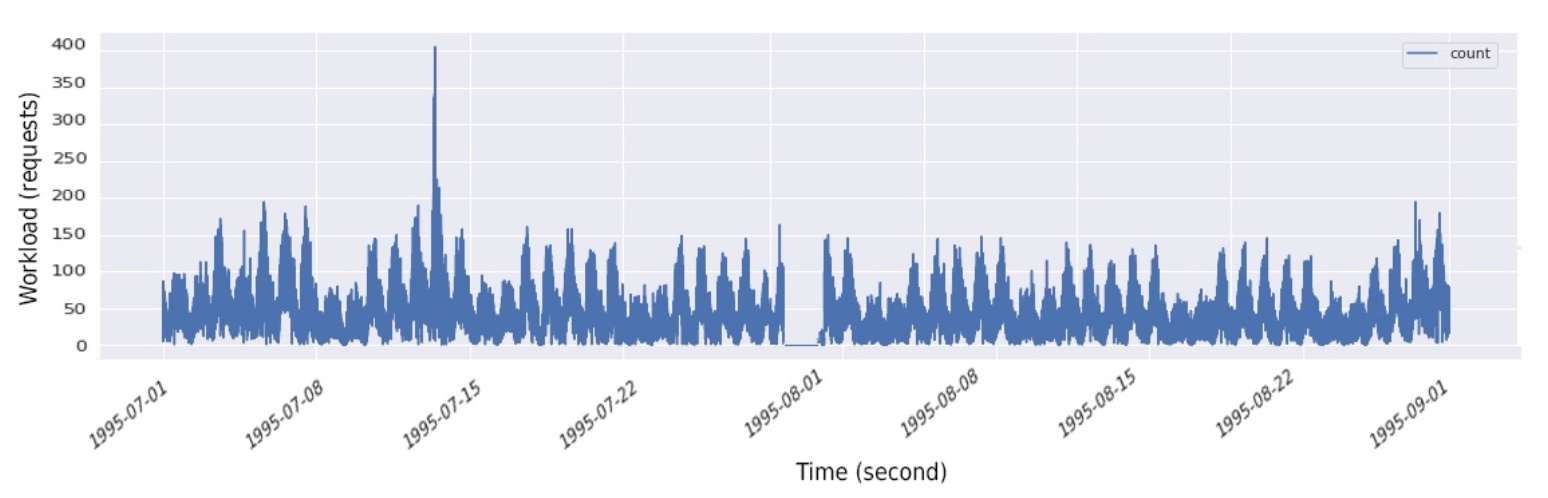
\includegraphics[width=1\textwidth]{chapter-4/nasa-aggr.png}
  \caption{Agregat Log \textit{Web Server} NASA}
  \label{fig:nasa-aggr}
\end{figure}

Untuk melakukan pengujian, karena pengujian ini sudah berbeda jauh dari alur utama sistem \textit{autoscaler}, maka khusus pengujian ini dilakukan pada program sendiri yang hanya akan melakukan \textit{training} serta prediksi untuk dievaluasi. Pertama-tama, data akan dibagi menjadi 70\% untuk \textit{training} dan 30\% untuk \textit{testing}. Akan dilakukan dua buah eksperimen, yaitu mengambil 10 menit terakhir dari data \textit{training} untuk melakukan prediksi 1 menit ke depan, dan mengambil 10 menit terakhir dari data \textit{training} untuk melakukan prediksi 5 menit ke depan. Konfigurasi $p$, $d$, dan $q$ akan dipilih oleh Auto ARIMA.

\subsubsection{Evaluasi}
% To evaluate the accuracy of the proposed model, we used four metrics as shown in Equations (6)–(9), respectively. These metrics are used to compare the prediction accuracies of the models. We define Yi as the actual value, Yˆ i as the forecast value, and Y ̄ i as the mean value of Y. In addition, we also compare the average prediction speed of 30 tries that each model takes for prediction.
% The mean square error (MSE) in Equation (6) calculates the average squared dif- ference between the forecast and the observed values. The root mean square error (RMSE), expressed as Equation (7), represents the square root of two of the differences between the forecast and observed values. The mean absolute error (MAE), expressed as Equation (8), represents the average over the test sample of the absolute differences between the prediction and actual observation, where all individual differences have equal weights. The metrics MSE, RMSE, MAE are used to evaluate the prediction error of the models, where a smaller value indicates a higher prediction accuracy and vice versa. The coefficient of determination, denoted as R2, is shown in Equation (9) as a goodness-of-fit measure for linear regression models. It is the square of the coefficients of multiple correlations between the observed outcomes and the observed predictor values. The higher the R2, the better the model fits the data.

Untuk melakukan evaluasi akurasi dari model yang digunakan, maka akan digunakan metrik sebagai berikut.

\begin{enumerate}
  \item \textbf{\textit{Mean Square Error (MSE)}}

        Metrik ini akan digunakan untuk mengkalkulasi rata-rata kuadrat dari selisih antara nilai prediksi dan nilai aktual. Semakin kecil nilai MSE, maka semakin baik model yang digunakan. Metrik ini didefinisikan pada persamaan \ref{eq:mse}. Dengan $Y_i$ adalah nilai aktual dan $\hat{Y_i}$ adalah nilai prediksi.

        \begin{equation}
          \label{eq:mse}
          MSE = \frac{1}{n}\sum_{i=1}^{n}(Y_i-\hat{Y}_i)
        \end{equation}

  \item \textbf{\textit{Root Mean Square Error (RMSE)}}

        RMSE, yang dituliskan pada persamaan \ref{eq:rmse}, merupakan akar kuadrat dari MSE.

        \begin{equation}
          \label{eq:rmse}
          RMSE = \sqrt{MSE} = \sqrt{\frac{1}{n}\sum_{i=1}^{n}(Y_i-\hat{Y}_i)}
        \end{equation}

  \item \textbf{\textit{Mean Absolute Error (MAE)}}

        MAE akan merepresentasikan rata-rata sampel uji dari perbedaan absolut antara prediksi dan pengamatan aktual. Metrik ini didefinisikan dengan persamaan \ref{eq:mae}.

        \begin{equation}
          \label{eq:mae}
          MAE = \frac{1}{n}\sum_{i=1}^{n}|(Y_i-\hat{Y_i})|
        \end{equation}

  \item \textbf{\textit{Coefficient of Determination ($R^{2}$)}}

        \textit{Coefficient of Determination} adalah ukuran \textit{good-of-fit} untuk model regresi linier yang didefinisikan dengan kuadrat dari koefisien korelasi antara hasil yang diamati dan nilai prediksi. Semakin tinggi R2, semakin model sesuai dengan data. $\bar{Y_i}$ adalah nilai rata-rata dari $Y$.

        \begin{equation}
          \label{eq:r2}
          R^{2} = 1-\frac{\sum_{i=1}^{n}(Y_i-\hat{Y_i})^{2}}{\sum_{i=1}^{n}(Y_i-\bar{Y_i})^{2}}
        \end{equation}
\end{enumerate}

MSE, RMSE, dan MAE akan digunakan untuk mengevaluasi eror pada hasil prediksi sedangkan $R^{2}$ akan digunakan untuk melakukan evaluasi \textit{good-of-fit} dari model. Semakin kecil MSE, RMSE, dan MAE maka akurasi model akan semakin bagus. Sedangkan semakin tinggi $R^{2}$ maka model akan semakin sesuai dengan data.

\subsubsection{Hasil Pengujian dan Analisis}

Setelah dilakukan pengujian, maka didapatkan angka berikut. Diambil juga data riset dengan eksperimen serupa dari \parencite{riset1} untuk sebagai perbandingan dengan Bi-LSTM. Perbandingan pengujian dengan model ARIMA dan Bi-LSTM  dapat dilihat pada tabel \ref{tab:pengujian-model-arima-bilstm}.

\begin{longtable}{|p{0.8in}|p{0.5in}|p{0.5in}|p{0.5in}|p{0.5in}|}

  \caption{Tabel Pengujian Model} \label{tab:pengujian-model-arima-bilstm}                                                                                                                                                                                   \\

  \hline
  \rowcolor{gray!30}\multicolumn{1}{|c|}{\textbf{Metrik}} & \multicolumn{1}{|c|}{\textbf{ARIMA 1 Step}} & \multicolumn{1}{|c|}{\textbf{ARIMA 5 Step}} & \multicolumn{1}{|c|}{\textbf{Bi-LSTM 1 Step}} & \multicolumn{1}{|c|}{\textbf{Bi-LSTM 5 Step}}        \\
  \hline
  \endfirsthead
  %
  \endhead
  %
  \multicolumn{1}{|c|}{MSE}                               & \multicolumn{1}{|c|}{196.288}               & \multicolumn{1}{|c|}{237.604}               & \multicolumn{1}{|c|}{183.642}                 & \multicolumn{1}{|c|}{207.313} \tabularnewline \hline

  \multicolumn{1}{|c|}{RMSE}                              & \multicolumn{1}{|c|}{14.010}                & \multicolumn{1}{|c|}{15.414}                & \multicolumn{1}{|c|}{13.551}                  & \multicolumn{1}{|c|}{14.39} \tabularnewline \hline

  \multicolumn{1}{|c|}{MAE}                               & \multicolumn{1}{|c|}{10.572}                & \multicolumn{1}{|c|}{11.628}                & \multicolumn{1}{|c|}{10.280}                  & \multicolumn{1}{|c|}{10.592} \tabularnewline \hline

  \multicolumn{1}{|c|}{$R^{2}$}                           & \multicolumn{1}{|c|}{0.692}                 & \multicolumn{1}{|c|}{0.628}                 & \multicolumn{1}{|c|}{0.712}                   & \multicolumn{1}{|c|}{0.675} \tabularnewline \hline

  Avg. Prediction Time (ms)                               & \multicolumn{1}{|c|}{2300}                  & \multicolumn{1}{|c|}{2488}                  & \multicolumn{1}{|c|}{4.3}                     & \multicolumn{1}{|c|}{45.1} \tabularnewline

  \hline
\end{longtable}

Dilakukan juga pembuatan grafik perbandingan nilai aktual dengan prediksi yang dapat dilihat pada gambar \ref{fig:arima-actual-predict}.

\begin{figure}[ht]
  \centering
  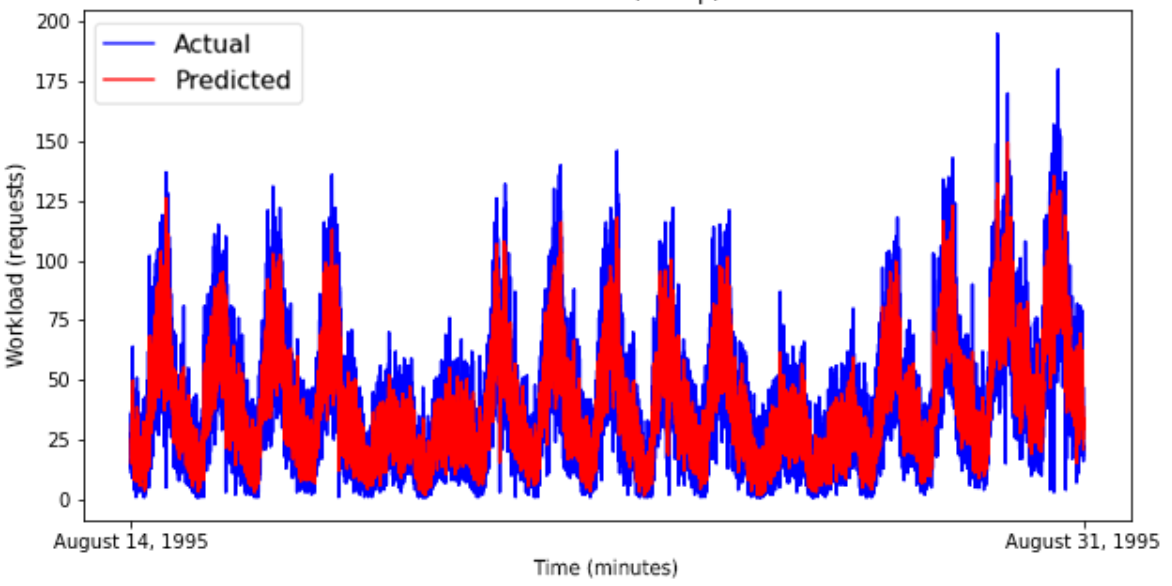
\includegraphics[width=1\textwidth]{chapter-4/arima-actual-predict.png}
  \caption{Perbandingan Nilai Aktual dan Prediksi Model ARIMA}
  \label{fig:arima-actual-predict}
\end{figure}

Model ARIMA bisa dipakai untuk melakukan prediksi dan dapat digunakan komponen \textit{Predictor} untuk melakukan prediksi. Sesuai yang sudah dibahas sebelumnya, mengincar kesederhanaan dengan \textit{trade-off} berupa kecepatan dan sedikit akurasi sudah sesuai dengan hasil pengujian ini.